%!TEX program = xelatex
% 完整编译: xelatex -> biber/bibtex -> xelatex -> xelatex
\documentclass[lang=cn,11pt,a4paper]{elegantpaper}

\usepackage{algorithm}
\usepackage[noend]{algpseudocode}
\usepackage{amsmath}
\usepackage{array}
\usepackage{xcolor}
\usepackage{graphicx}

\lstdefinelanguage{text}{
    showstringspaces=false,
    breaklines=true,
    breakatwhitespace=true,
    tabsize=4
}

\title{《算法设计与分析》\\课程实验报告}

\author{
\huge 专业:计算机科学与技术 \\[10pt]
\huge 班级:2021211304 \\[10pt]
\huge 姓名:杨晨 \\[10pt]
\huge 学号:2021212171
}
\date{}

% 本文档命令
\usepackage{array}
\newcommand{\ccr}[1]{\makecell{{\color{#1}\rule{1cm}{1cm}}}}

\begin{document}

\maketitle

\clearpage

% \begin{abstract}
% 本文为 \href{https://github.com/ElegantLaTeX/ElegantPaper/}{ElegantPaper} 的说明文档。此模板基于 \LaTeX{} 的 article 类,专为工作论文写作而设计。设计这个模板的初衷是让作者不用关心工作论文的格式,专心写作,从而有更加舒心的写作体验。如果你有其他问题、建议或者报告 bug,可以在 \href{https://github.com/ElegantLaTeX/ElegantPaper/issues}{GitHub::ElegantPaper/issues} 留言。如果你想了解更多 Elegant\LaTeX{} 项目组设计的模板,请访问 \href{https://github.com/ElegantLaTeX/}{GitHub::ElegantLaTeX}。
% \keywords{Elegant\LaTeX{},工作论文,模板}
% \end{abstract}


\section{概述}

\subsection{实验内容}

\begin{itemize}
    \item 二选一,编程实现下述算法
    \begin{itemize}
        \item 线性时间选择
        \item 平面最近点对
    \end{itemize}
    \item 利用
    \begin{itemize}
        \item xx省会城市TD-LTE网络的小区/基站数据,针对线性时间选择、平面最近点对,验证算法正确性,观察分析算法的时间、空间复杂性变化
    \end{itemize}
\end{itemize}

\subsection{开发环境}

\begin{itemize}
    \item Windows10
    \item PyCharm 2023.2.4 (Professional Edition)
\end{itemize}

\section{实验过程}

\subsection{线性时间选择}

\subsubsection{介绍}

选择问题涉及在一个无序的包含$n$个元素的列表中找到第$k$小的元素。解决这个问题的朴素方法是对列表进行排序,然后返回第$k$个元素。然而,这种方法使用基于比较的排序算法(如快速排序或归并排序)的时间复杂度为$O(n \log n)$。

线性时间选择算法,也称为\textit{快速选择}算法,提供了一个高效的解决方案,平均时间复杂度为$O(n)$。它基于快速排序中的划分技术。

\subsubsection{算法描述}

快速选择算法通过从列表中选择一个枢轴元素,并围绕枢轴将元素进行划分,使得所有小于枢轴的元素在其左侧,所有大于枢轴的元素在其右侧。这个过程类似于快速排序中的划分步骤。

中位数法选择枢轴是一种优化策略,它确保了良好的枢轴选择,从而避免了最坏情况的发生。该方法的步骤如下:
\begin{enumerate}
  \item 将列表划分为大小为5的子列表(最后一个子列表的大小可以小于5)。
  \item 对每个子列表进行排序。
  \item 从每个子列表中选择中位数,将这些中位数组成一个新的列表。
  \item 递归地应用快速选择算法来选择新列表的中位数作为枢轴。
\end{enumerate}

算法继续使用快速选择的步骤,根据枢轴将列表划分为左、右两个部分,并根据$k$的值进行递归搜索。如果枢轴元素是第$k$个元素,我们找到了所需的值并返回它。否则,我们根据$k$是小于还是大于枢轴的索引,在左侧或右侧划分上递归应用算法。

快速选择算法的伪代码如算法\ref{alg:quickselect}所示。

\begin{algorithm}
\caption{快速选择算法}\label{alg:quickselect}
\begin{algorithmic}
\Function{QuickSelect}{A, low, high, k}
  \State{$pivot \gets$ 中位数法选择枢轴($A$)} \Comment{使用中位数法选择一个枢轴元素}
  \State{交换$A[low]$和$pivot$} \Comment{将枢轴元素放到开头}
  \State{$mid \gets$ \Call{Partition}{$A, low, high$}} \Comment{调用 Partition 函数}
  \If{$mid-low+1 == k$}
    \State{\textbf{return} $A[mid]$} \Comment{找到第$k$个元素}
  \ElsIf{$mid-low+1 > k$}
    \State{\textbf{return} \textsc{Quickselect}($A, low, mid-1, k$)} \Comment{在左侧划分中递归搜索}
  \Else
    \State{\textbf{return} \textsc{Quickselect}($A, mid+1, high, k-(mid - low + 1)$)} \Comment{在右侧划分中递归搜索}
  \EndIf
\EndFunction

\Function{Partition}{$A, low, high$}
  \State{$pivot \gets A[low]$} \Comment{以列表开头元素划分}
  \State{$i \gets low + 1$}
  \State{$j \gets high$}
  
  \While{\textbf{True}} \Comment{按照枢轴元素进行划分,同快速排序}
    \While{$i \leq j$ \textbf{并且} $A[i] \leq pivot$}
      \State{$i \gets i + 1$}
    \EndWhile
    
    \While{$i \leq j$ \textbf{并且} $A[j] \geq pivot$}
      \State{$j \gets j - 1$}
    \EndWhile
    
    \If{$i > j$}
      \State{\textbf{break}}
    \EndIf
    
    \State{交换$A[i]$和$A[j]$}
  \EndWhile
  
  \State{交换$A[low]$和$A[j]$}
  \State{\textbf{return} $j$} \Comment{返回枢轴元素下标}
\EndFunction
\end{algorithmic}
\end{algorithm}


\subsubsection{分析}
快速选择算法的平均时间复杂度为$O(n)$,通过使用中位数法选择枢轴,可以避免最坏情况的发生,确保算法的时间复杂度为$O(n)$。中位数法选择枢轴的时间复杂度为$O(n)$,因为它涉及对子列表进行排序和选择中位数。

选择问题的最坏情况发生在每次划分都产生极度不平衡的子列表时,这时快速选择算法的时间复杂度可能达到$O(n^2)$。然而,通过使用中位数法选择枢轴,我们可以减少最坏情况的概率,并获得平均时间复杂度为$O(n)$的性能。

\subsubsection{运行结果}
\begin{lstlisting}[language=text]
最小的元素为: 103.075
递归最大层次为: 7 

第5小的元素为: 126.096
递归最大层次为: 7 

第50小的元素为: 208.475
递归最大层次为: 7 

最大的元素为: 2735.798
递归最大层次为: 7 

通过排序验证结果的正确性:
最小的元素为: 103.075
第5小的元素为: 126.096
第50小的元素为: 208.475
最大的元素为: 2735.798
\end{lstlisting}

\subsubsection{结论}
线性时间选择算法,即快速选择算法,为选择问题提供了高效的解决方案。通过利用快速排序中的划分技术和中位数法选择枢轴,它实现了平均时间复杂度为$O(n)$,因此在查找无序列表中第$k$小的元素时是一个很好的选择。中位数法选择枢轴可以避免最坏情况的发生,确保算法的性能始终为$O(n)$。快速选择算法在实践中被广泛应用于各种需要选择问题的场景中,提供了高效的解决方案。

\subsection{最近平面点对}

\subsubsection{介绍}
给定平面上的 $n$ 个点 $P = \{p_0, p_2, \ldots, p_{n-1}\}$,其中每个点 $p_i$ 的坐标表示为 $(x_i, y_i)$。最近平面点对问题要求找到两个点 $p_i$ 和 $p_j$,使得它们的欧氏距离 $d(p_i, p_j)$ 最小,即 $d(p_i, p_j) = \sqrt{(x_i-x_j)^2 + (y_i-y_j)^2}$。

\subsubsection{算法描述}
最近平面点对算法采用分治法的思想来提高效率。分治法的基本思路是,将大问题转化为类似的小问题,解决小问题后通过合并解决大问题。在本题中,我们要解决的问题就是计算标号为$1,2\dots(n -1)$的这$n$个点的两点间最近距离。我们设计算标号为$l,l+1\dots(r -1)$的点的两点间最近距离为$f(l,r)$,最终目标即求$f(0,n)$。要想解决$f(l,r)$,可以考虑先解决$f(l,\left\lfloor \frac{l+r}{2} \right\rfloor)$和$f(\left\lfloor \frac{l+r}{2} \right\rfloor,r)$

容易发现,当$r=l+1$时不需要做任何处理(此时返回$\infty$)。关键问题在于,如何合并两个子问题的结果。
\begin{enumerate}
    \item 记$d$为左右区间的最小距离,找到左右两部分的中线$mid=l+\frac{r-l}{2}$,此时只需要在横坐标$x\in(mid-d,mid+d)$的区间中找即可
    \item 对所有横坐标$x\in(mid-d,mid+d)$的点按照$y$排序,我们只需要考虑$y_j-y_i<d(i<j)$的点对
\end{enumerate}

所以,合并时,中线附近的点,只需要考虑的范围是一个长为$2d$宽为$d$的矩形。容易证明,这个区域内最多扫描六个点

\begin{figure}[!htb]
\centering
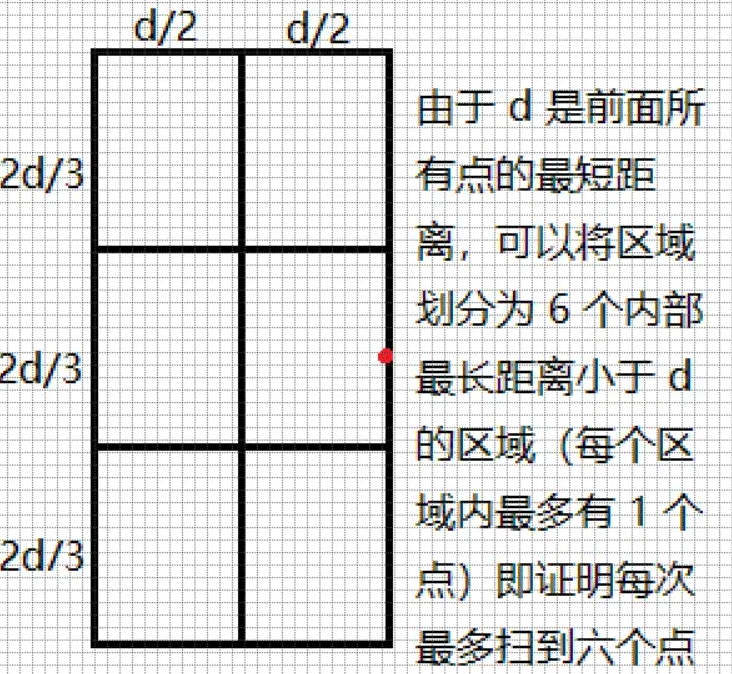
\includegraphics[width=0.5\textwidth]{image/near.png}
\end{figure}

\[
\begin{aligned}
\sqrt{{\frac{1}{2}}^2 + {\frac{2}{3}}^2}=\frac{5}{6} < 1
\end{aligned}
\]

最近平面点对算法的伪代码如算法\ref{alg:NearestPair}所示

\begin{algorithm}
\caption{NearestPair}\label{alg:NearestPair}
\begin{algorithmic}
\Function{Merge}{$stations, l, mid, r$}
    \Comment{合并两个有序数组,区间$[l,\text{mid})$和$[\text{mid},r)$,按照$y$坐标排序}
    \State merged $\gets$ sorted(stations[l:r], $\lambda \text{station}: \text{station.y}$)
    \State stations[l:r] $\gets$ merged
\EndFunction

\Function{NearestPair}{$stations, l, r, min\_dis, lesser\_dis$}
    \Comment{求解最近点对,区间为$[l,r)$}
    \If{$r - l \leq 1$}
        \State \Return min\_dis, lesser\_dis
    \EndIf
    \State mid $\gets$ l + (r - l) $\div$ 2
    \Comment{递归求解左右两边的最近点对}
    \State min\_dis, lesser\_dis $\gets$ \text{NearestPair}(stations, l, mid, \text{min\_dis}, \text{lesser\_dis})
    \State min\_dis, lesser\_dis $\gets$ \text{NearestPair}(stations, mid, r, \text{min\_dis}, \text{lesser\_dis})
    \State \text{Merge}(stations, l, mid, r)
    \Comment{合并两个有序数组,按照$y$坐标排序}
    \State mid\_line $\gets$ stations[mid].x
    \Comment{中线}
    \State selected $\gets$ []
    \For{i $\gets$ l to r}
        \If{$|\text{stations[i].x} - \text{mid\_line}| < \text{min\_dis}[0]$}
            \State \text{selected.append(stations[i])}
        \EndIf
    \EndFor
    \For{i $\gets$ 0 to len(selected) - 1}
        \For{j $\gets$ i + 1 to len(selected)}
            \If{selected[j].y - selected[i].y $\geq$ min\_dis[0]}
                \State \text{break}
            \EndIf
            \State dis $\gets$ \text{calculate\_distance}(selected[i].y, selected[i].x, selected[j].y, selected[j].x)
            \If{dis = 0}
                \State \text{continue}
            \EndIf
            \If{dis < min\_dis[0]}
                \Comment{更新最近点对}
                \State lesser\_dis $\gets$ min\_dis
                \State min\_dis $\gets$ (dis, selected[i].eNodeB\_id, selected[j].eNodeB\_id)
            \ElsIf{min\_dis[0] < dis < lesser\_dis[0]}
                \Comment{更新次近点对}
                \State lesser\_dis $\gets$ (dis, selected[i].eNodeB\_id, selected[j].eNodeB\_id)
            \EndIf
        \EndFor
    \EndFor
    \State \Return min\_dis, lesser\_dis
\EndFunction
\end{algorithmic}
\end{algorithm}

\subsubsection{分析}
最近平面点对算法的时间复杂度为 $O(n \log n)$,空间复杂度为 $O(n)$。以下是对算法性能的进一步分析:

\begin{itemize}
  \item 算法的主要开销在于对点集的排序以及递归过程中的计算。
  \item 排序点集的时间复杂度为 $O(n \log n)$,可以使用快速排序或归并排序等常见排序算法实现。
  \item 递归过程中,每次将点集划分为两部分,并在每个子问题中计算最近点对,因此总共需要进行 $O(\log n)$ 层递归。
  \item 在每层递归中,计算最近点对的时间复杂度为 $O(n)$。
\end{itemize}

\clearpage

\subsubsection{运行结果}
\begin{lstlisting}[language=text]
最近点对距离为: 1.278655 ,eNodeB_id分别为: 567389 566803
次近点对距离为: 1.673381 ,eNodeB_id分别为: 567222 566784

通过遍历求解的结果:
最近点对距离为: 1.278655 ,eNodeB_id分别为: 566803 567389
次近点对距离为: 1.673381 ,eNodeB_id分别为: 566784 567222
\end{lstlisting}

\subsubsection{结论}
最近平面点对算法是一种高效的方法,用于解决平面上最接近的点对问题。通过使用分治法和合适的数据结构,可以在较短的时间内找到最近点对。该算法在计算几何学和计算机图形学等领域有广泛应用。

\section{附录:完整代码}

\subsection{线性时间选择}
\begin{lstlisting}[language=python]
import pandas as pd


def bubble_sort(arr, low, high):
    """
    冒泡排序
    :param arr: 待排序列表
    :param low: 左边界
    :param high: 右边界
    :return: 从低到高排序的列表
    """
    n = high - low + 1
    for i in range(n):
        is_swapped = False
        for j in range(n - i - 1):
            if arr[j + low] > arr[j + 1 + low]:
                arr[j + low], arr[j + 1 + low] = arr[j + 1 + low], arr[j + low]
                is_swapped = True
        if not is_swapped:
            break


# 全局变量,记录选择划分过程的递归层次
recursion_level = 0


def clear_level():
    """
    将递归层次清零
    :return:
    """
    global recursion_level
    recursion_level = 0


def linear_select(arr, low, high, k, current_level=1):
    """
    线性时间选择算法
    :param arr:待划分数组
    :param low: 左边界
    :param high: 右边界
    :param k: 选择的第k小的元素
    :return:
    """
    global recursion_level
    recursion_level = max(recursion_level, current_level)
    if high - low + 1 < 20:
        # 如果数组长度小于20,则直接排序
        bubble_sort(arr, low, high)
        return arr[low + k - 1]

    # 5个元素一组,分别排序
    for i in range(low, high - 4, 5):
        bubble_sort(arr, i, i + 4)
        # 将中位数放到数组最前面
        arr[low + (i - low) // 5], arr[i + 2] = arr[i + 2], arr[low + (i - low) // 5]
    # 得到中位数的中位数
    cnt = (high - low + 1) // 5
    pivot = linear_select(arr, low, low + cnt - 1, cnt // 2 + 1, current_level + 1)
    # 得到pivot的下标
    pivot = arr.index(pivot)
    # 将pivot放到数组最前面
    arr[low], arr[pivot] = arr[pivot], arr[low]
    # 一分为三
    pivot = partition_three(arr, low, high)
    # 递归寻找
    if pivot - low + 1 == k:
        return arr[pivot]
    elif pivot - low + 1 > k:
        return linear_select(arr, low, pivot - 1, k, current_level + 1)
    else:
        return linear_select(
            arr, pivot + 1, high, k - (pivot - low + 1), current_level + 1
        )


def partition_three(arr, low, high):
    """
    一分为三,基准元素为数组第一个元素
    :param arr:待划分数组
    :param low: 左边界
    :param high: 右边界
    :return: 划分后基准元素的下标
    """
    pivot = arr[low]
    # 将数组分为三部分
    i = low + 1
    j = high
    while True:
        while i <= j and arr[i] <= pivot:
            i += 1
        while i <= j and arr[j] >= pivot:
            j -= 1
        if i > j:
            break
        arr[i], arr[j] = arr[j], arr[i]
    arr[low], arr[j] = arr[j], arr[low]
    return j


if __name__ == "__main__":
    # 读取基站数据文件
    data = pd.read_excel(
        r"C:\Users\Administrator\Desktop\算法设计与分析-编程作业-第2章 分治-2023\02-1 1033个基站数据.xls"
    )
    # 删除未命名的列
    data = data.loc[:, ~data.columns.str.contains("^Unnamed")]

    # 提取k-dist列的数据
    k_dist_values = data["K_DIST"].tolist()
    k_dist_copy = k_dist_values.copy()  # 复制一份用于验证结果的正确性

    # 选择最小的元素
    min_dist_values = linear_select(k_dist_values, 0, len(k_dist_values) - 1, 1)
    print("最小的元素为:", min_dist_values)
    print("递归最大层次为:", recursion_level, "\n")

    # 选择第5小的元素
    clear_level()
    min_dist_values = linear_select(k_dist_values, 0, len(k_dist_values) - 1, 5)
    print("第5小的元素为:", min_dist_values)
    print("递归最大层次为:", recursion_level, "\n")

    # 选择第50小的元素
    clear_level()
    min_dist_values = linear_select(k_dist_values, 0, len(k_dist_values) - 1, 50)
    print("第50小的元素为:", min_dist_values)
    print("递归最大层次为:", recursion_level, "\n")

    # 选择最大的元素
    clear_level()
    min_dist_values = linear_select(
        k_dist_values, 0, len(k_dist_values) - 1, len(k_dist_values)
    )
    print("最大的元素为:", min_dist_values)
    print("递归最大层次为:", recursion_level, "\n")

    # 验证结果的正确性
    k_dist_copy.sort()
    print("通过排序验证结果的正确性:")
    print("最小的元素为:", k_dist_copy[0])
    print("第5小的元素为:", k_dist_copy[4])
    print("第50小的元素为:", k_dist_copy[49])
    print("最大的元素为:", k_dist_copy[-1])

\end{lstlisting}

\subsection{最近平面点对}
\begin{lstlisting}[language=python]
import numpy as np
import pandas as pd


def degree_to_radian(degree):
    """
    将给定的经纬度转化为弧度
    :param degree: 1个输入(经纬度)
    :return: 转化为的弧度
    """
    return degree * np.pi / 180


def calculate_distance(lat1, lon1, lat2, lon2):
    """
    距离公式
    :param lat1: 纬度1
    :param lon1: 经度1
    :param lat2: 纬度2
    :param lon2: 经度2
    :return: 距离/m,保留6位小数
    """
    if abs(lat1 - lat2) < 1e-6 and abs(lon1 - lon2) < 1e-6:
        return 0
    rad_lat1 = degree_to_radian(lat1)
    rad_lon1 = degree_to_radian(lon1)
    rad_lat2 = degree_to_radian(lat2)
    rad_lon2 = degree_to_radian(lon2)
    # R为赤道半径/m
    R = 6378.137 * 1000
    dis = R * np.arccos(
        np.cos(rad_lat1) * np.cos(rad_lat2) * np.cos(rad_lon1 - rad_lon2)
        + np.sin(rad_lat1) * np.sin(rad_lat2)
    )
    return round(dis, 6)


class Station:
    def __init__(self, eNodeB_id, latitude, longitude):
        self.eNodeB_id = eNodeB_id
        self.x = longitude
        self.y = latitude


def merge(stations, l, mid, r):
    """
    合并两个有序数组,区间[l,mid)和[mid,r),但是按照y坐标排序
    :param stations: 基站列表
    :param l: 左边界
    :param mid: 中间位置
    :param r: 右边界
    """
    merged = sorted(stations[l:r], key=lambda station: station.y)
    stations[l:r] = merged


def nearest_pair(stations, l, r, min_dis, lesser_dis):
    """
    求解最近点对,区间为[l,r)
    :param stations: 基站列表
    :param l: 左边界
    :param r: 右边界
    :param min_dis: 最近距离 (距离,eNodeB_id1,eNodeB_id2)
    :param lesser_dis: 次近距离 (距离,eNodeB_id1,eNodeB_id2)
    :return: 最近距离 (距离,eNodeB_id1,eNodeB_id2),次近距离 (距离,eNodeB_id1,eNodeB_id2)
    """
    if r - l <= 1:
        return min_dis, lesser_dis
    mid = l + (r - l) // 2
    # 递归求解左右两边的最近点对
    min_dis, lesser_dis = nearest_pair(stations, l, mid, min_dis, lesser_dis)
    min_dis, lesser_dis = nearest_pair(stations, mid, r, min_dis, lesser_dis)
    # 合并两个有序数组,但是按照y坐标排序
    merge(stations, l, mid, r)
    # 选取中间区域的点
    mid_line = stations[mid].x  # 中线
    selected = []
    for i in range(l, r):  # 选取中线左右两边距离中线小于min_dis的点
        if abs(stations[i].x - mid_line) < min_dis[0]:
            selected.append(stations[i])
    # 计算最近点对
    for i in range(len(selected)):
        for j in range(i + 1, len(selected)):
            if selected[j].y - selected[i].y >= min_dis[0]:  # 剪枝,y距离大于min_dis的点不用计算
                break
            dis = calculate_distance(
                selected[i].y, selected[i].x, selected[j].y, selected[j].x
            )
            if dis == 0:  # 剪枝,距离为0的点对不用计算
                continue
            if dis < min_dis[0]:  # 更新最近点对
                lesser_dis = min_dis
                min_dis = (dis, selected[i].eNodeB_id, selected[j].eNodeB_id)
            elif min_dis[0] < dis < lesser_dis[0]:  # 更新次近点对
                lesser_dis = (dis, selected[i].eNodeB_id, selected[j].eNodeB_id)

    return min_dis, lesser_dis


if __name__ == "__main__":
    # 读取基站数据文件
    data = pd.read_excel(
        r"C:\Users\Administrator\Desktop\算法设计与分析-编程作业-第2章 分治-2023\02-1 1033个基站数据.xls"
    )
    # 删除未命名的列
    data = data.loc[:, ~data.columns.str.contains("^Unnamed")]

    eNodeB_id = data["ENODEBID"].tolist()
    longitude = data["LONGITUDE"].tolist()
    latitude = data["LATITUDE"].tolist()

    # 创建对象的列表
    stations = [
        Station(eNodeB_id, lon, lat)
        for eNodeB_id, lon, lat in zip(eNodeB_id, longitude, latitude)
    ]
    stations_copy = stations.copy()  # 复制一份用于验证结果的正确性

    min_dis = (1e10, -1, -1)
    lesser_dis = (1e10, -1, -1)

    stations.sort(key=lambda station: station.x)

    # 求解最近点对
    min_dis, lesser_dis = nearest_pair(stations, 0, len(stations), min_dis, lesser_dis)
    print("最近点对距离为:", min_dis[0], ",eNodeB_id分别为:", min_dis[1], min_dis[2])
    print("次近点对距离为:", lesser_dis[0], ",eNodeB_id分别为:", lesser_dis[1], lesser_dis[2])

    # 验证结果的正确性
    min_dis_ = 1e10
    lesser_dis_ = 1e10
    min_id1, min_id2, lesser_id1, lesser_id2 = -1, -1, -1, -1
    for i in range(len(stations_copy)):
        for j in range(i + 1, len(stations_copy)):
            dis = calculate_distance(
                stations_copy[i].y,
                stations_copy[i].x,
                stations_copy[j].y,
                stations_copy[j].x,
            )
            if dis == 0:  # 剪枝,距离为0的点对不用计算
                continue
            if dis < min_dis_:
                lesser_dis_ = min_dis_
                lesser_id1, lesser_id2 = min_id1, min_id2
                min_dis_ = dis
                min_id1, min_id2 = (
                    stations_copy[i].eNodeB_id,
                    stations_copy[j].eNodeB_id,
                )
            elif min_dis_ < dis < lesser_dis_:
                lesser_dis_ = dis
                lesser_id1, lesser_id2 = (
                    stations_copy[i].eNodeB_id,
                    stations_copy[j].eNodeB_id,
                )
    print("\n通过遍历求解的结果:")
    print("最近点对距离为:", min_dis_, ",eNodeB_id分别为:", min_id1, min_id2)
    print("次近点对距离为:", lesser_dis_, ",eNodeB_id分别为:", lesser_id1, lesser_id2)

\end{lstlisting}

% 时隔两年,本模板迎来更新,中间发生了很多变化,两个主要变化是参考文献与字体设定,\textbf{使用前请务必仔细阅读本文档}。

% \textbf{文献部分}:我们将 bibtex 的默认文献编译方式改为 biblatex,不过我们也提供了两个后端,\lstinline{bibend=biber} 和 \lstinline{bibend=bibtex}。特别需要注意的是,从 0.10 开始,文献文件改为 \lstinline{reference.bib},与 ElegantBook 保持一致,而参考文献的引文样式等更多格式,请参考后文参考文献部分,更多样式可以参考 biblatex 文档。 

% \textbf{字体部分},我们将 newtxtext 宏包的支持方式改为了字体名称设定方式,设定英文字体为 TeX Gyre Terms/Heros,,英文字体部分,根据编译方式选择不同字体。对于一般用户而言,不太需要关心这部分内容。

% 另外,中文请务必使用 \hologo{XeLaTeX} 编译。

% \subsection{模板介绍}

% 此模板基于 \LaTeX{} 的标准文类 article 设计,所以 article 文类的选项也能传递给本模板,比如 \lstinline{a4paper, 11pt} 等等。

% \begin{lstlisting}
% \documentclass[a4paper,11pt]{elegantpaper}
% \end{lstlisting}

% \textbf{注意}:Elegant\LaTeX{} 系列模板已经全部上传至 \href{https://www.overleaf.com/latex/templates/elegantpaper-template/yzghrqjhmmmr}{Overleaf} 上,用户可以在线使用。另外,为了方便国内用户,模板也已经传至\href{https://gitee.com/ElegantLaTeX/ElegantPaper}{码云}。


% \subsection{全局选项}
% 此模板定义了一个语言选项 \lstinline{lang},可以选择英文模式 \lstinline{lang=en}(默认)或者中文模式 \lstinline{lang=cn}。当选择中文模式时,图表的标题引导词以及参考文献,定理引导词等信息会变成中文。你可以通过下面两种方式来选择语言模式:
% \begin{lstlisting}
% \documentclass[lang=cn]{elegantpaper} % or
% \documentclass{cn}{elegantpaper} 
% \end{lstlisting}

% \textbf{注意:} 英文模式下,由于没有添加中文宏包,无法输入中文。如果需要输入中文,可以通过在导言区引入中文宏包 \lstinline{ctex} 或者加入 \lstinline{xeCJK} 宏包后自行设置字体。 
% \begin{lstlisting}
% \usepackage[UTF8,scheme=plain]{ctex}
% \end{lstlisting}

% \subsection{数学字体选项}

% 本模板定义了一个数学字体选项(\lstinline{math}),可选项有三个:
% \begin{enumerate}
%   \item \lstinline{math=cm}(默认),使用 \LaTeX{} 默认数学字体(推荐,无需声明);
%   \item \lstinline{math=newtx},使用 \lstinline{newtxmath} 设置数学字体(潜在问题比较多)。
%   \item \lstinline{math=mtpro2},使用 \lstinline{mtpro2} 宏包设置数学字体,要求用户已经成功安装此宏包。
% \end{enumerate}

% \subsection{中文字体选项}

% 模板提供中文字体选项 \lstinline{chinesefont},可选项有
% \begin{enumerate}
%   \item \lstinline{ctexfont}:默认选项,使用 \lstinline{ctex} 宏包根据系统自行选择字体,可能存在字体缺失的问题,更多内容参考 \lstinline{ctex} 宏包\href{https://ctan.org/pkg/ctex}{官方文档}\footnote{可以使用命令提示符,输入 \lstinline{texdoc ctex} 调出本地 \lstinline{ctex} 宏包文档}。
%   \item \lstinline{founder}:方正字体选项(\textbf{需要安装方正字体}),后台调用 \lstinline{ctex} 宏包并且使用 \lstinline{fontset=none} 选项,然后设置字体为方正四款免费字体,方正字体下载注意事项见后文,用户只需要安装方正字体即可使用该选项。
%   \item \lstinline{nofont}:后台会调用 \lstinline{ctex} 宏包并且使用 \lstinline{fontset=none} 选项,不设定中文字体,用户可以自行设置中文字体,具体见后文。
% \end{enumerate}

% \subsubsection{方正字体选项}
% 由于使用 \lstinline{ctex} 宏包默认调用系统已有的字体,部分系统字体缺失严重,因此,用户希望能够使用其它字体,我们推荐使用方正字体。方正的{\songti 方正书宋}、{\heiti 方正黑体}、{\kaishu 方正楷体}、{\fangsong 方正仿宋}四款字体均可免费试用,且可用于商业用途。用户可以自行从\href{http://www.foundertype.com/}{方正字体官网}下载此四款字体,在下载的时候请\textbf{务必}注意选择 GBK 字符集,也可以使用 \href{https://www.latexstudio.net/}{\LaTeX{} 工作室}提供的\href{https://pan.baidu.com/s/1BgbQM7LoinY7m8yeP25Y7Q}{方正字体,提取码为:njy9} 进行安装。安装时,{\kaishu Win 10 用户请右键选择为全部用户安装,否则会找不到字体。}

% \begin{figure}[!htb]
% \centering
% 
\includegraphics[width=0.9\textwidth]{founder.png}
% \end{figure}

% \subsubsection{其他中文字体}
% 如果你想完全自定义字体\footnote{这里仍然以方正字体为例。},你可以选择 \lstinline{chinesefont=nofont},然后在导言区设置即可,可以参考下方代码:
% \begin{lstlisting}
% \setCJKmainfont[BoldFont={FZHei-B01},ItalicFont={FZKai-Z03}]{FZShuSong-Z01}
% \setCJKsansfont[BoldFont={FZHei-B01}]{FZKai-Z03}
% \setCJKmonofont[BoldFont={FZHei-B01}]{FZFangSong-Z02}
% \setCJKfamilyfont{zhsong}{FZShuSong-Z01}
% \setCJKfamilyfont{zhhei}{FZHei-B01}
% \setCJKfamilyfont{zhkai}[BoldFont={FZHei-B01}]{FZKai-Z03}
% \setCJKfamilyfont{zhfs}[BoldFont={FZHei-B01}]{FZFangSong-Z02}
% \newcommand*{\songti}{\CJKfamily{zhsong}}
% \newcommand*{\heiti}{\CJKfamily{zhhei}}
% \newcommand*{\kaishu}{\CJKfamily{zhkai}}
% \newcommand*{\fangsong}{\CJKfamily{zhfs}}
% \end{lstlisting}



% \subsection{自定义命令}
% 此模板并没有修改任何默认的 \LaTeX{} 命令或者环境\footnote{目的是保证代码的可复用性,请用户关注内容,不要太在意格式,这才是本工作论文模板的意义。}。另外,我自定义了 4 个命令:
% \begin{enumerate}
%   \item \lstinline{\email}:创建邮箱地址的链接,比如 \email{ddswhu@outlook.com};
%   \item \lstinline{\figref}:用法和 \lstinline{\ref} 类似,但是会在插图的标题前添加 <\textbf{图 n}> ;
%   \item \lstinline{\tabref}:用法和 \lstinline{\ref} 类似,但是会在表格的标题前添加 <\textbf{表 n}>;
%   \item \lstinline{\keywords}:为摘要环境添加关键词。
% \end{enumerate}

% \subsection{参考文献}

% 文献部分,本模板调用了 biblatex 宏包,并提供了 biber(默认) 和 bibtex 两个后端选项,可以使用 \lstinline{bibend} 进行修改:

% \begin{lstlisting}
%   \documentclass[bibtex]{elegantpaper}
%   \documentclass[bibend=bibtex]{elegantpaper}
% \end{lstlisting}

% 关于文献条目(bib item),你可以在谷歌学术,Mendeley,Endnote 中取,然后把它们添加到 \lstinline{reference.bib} 中。在文中引用的时候,引用它们的键值(bib key)即可。

% 为了方便文献样式修改,模板引入了 \lstinline{bibstyle} 和 \lstinline{citestyle} 选项,默认均为数字格式(numeric),参考文献示例:\cite{cn1,en2,en3} 使用了中国一个大型的 P2P 平台(人人贷)的数据来检验男性投资者和女性投资者在投资表现上是否有显著差异。

% 如果需要设置为国标 GB7714-2015,需要使用:
% \begin{lstlisting}
%   \documentclass[citestyle=gb7714-2015, bibstyle=gb7714-2015]{elegantpaper} 
% \end{lstlisting}

% 如果需要添加排序方式,可以在导言区加入
% \begin{lstlisting}
%   \ExecuteBibliographyOptions{sorting=ynt}
% \end{lstlisting}

% 启用国标之后,可以加入 \lstinline{sorting=gb7714-2015}。


% \section{使用 newtx 系列字体}

% 如果需要使用原先版本的 \lstinline{newtx} 系列字体,可以通过显示声明数学字体:

% \begin{lstlisting}
% \documentclass[math=newtx]{elegantpaper}
% \end{lstlisting}

% \subsection{连字符}

% 如果使用 \lstinline{newtx} 系列字体宏包,需要注意下连字符的问题。
% \begin{equation}
%   \int_{R^q} f(x,y) dy.\emph{of\kern0pt f}
% \end{equation}

% \begin{lstlisting}
% \begin{equation}
%   \int_{R^q} f(x,y) dy.\emph{of \kern0pt f}
% \end{equation}
% \end{lstlisting}

% \subsection{宏包冲突}

% 有用户反馈模板在使用 \lstinline{yhmath} 以及 \lstinline{esvect} 等宏包时会报错:
% \begin{lstlisting}
% LaTeX Error:
%    Too many symbol fonts declared.
% \end{lstlisting}

% 原因是在使用 \lstinline{newtxmath} 宏包时,重新定义了数学字体用于大型操作符,达到了 {\heiti 最多 16 个数学字体} 的上限,在调用其他宏包的时候,无法新增数学字体。为了减少调用非常用宏包,在此给出如何调用 \lstinline{yhmath} 以及 \lstinline{esvect} 宏包的方法。

% 请在 \lstinline{elegantpaper.cls} 内搜索 \lstinline{yhmath} 或者 \lstinline{esvect},将你所需要的宏包加载语句\textit{取消注释}即可。


% \section{常见问题 FAQ}

% \begin{enumerate}[label=\arabic*).]
%   \item \textit{如何删除版本信息?}\\
%     导言区不写 \lstinline|\version{x.xx}| 即可。
%   \item \textit{如何删除日期?}\\
%     需要注意的是,与版本 \lstinline{\version} 不同的是,导言区不写或注释 \lstinline{\date} 的话,仍然会打印出当日日期,原因是 \lstinline{\date} 有默认参数。如果不需要日期的话,日期可以留空即可,也即 \lstinline|\date{}|。
%   \item \textit{如何获得中文日期?}\\
%     为了获得中文日期,必须在中文模式下\footnote{英文模式下,由于未加载中文宏包,无法输入中文。},使用 \lstinline|\date{\zhdate{2019/10/11}}|,如果需要当天的汉化日期,可以使用 \lstinline|\date{\zhtoday}|,这两个命令都来源于 \href{https://ctan.org/pkg/zhnumber}{\lstinline{zhnumber}} 宏包。
%   \item \textit{如何添加多个作者?}\\
%     在 \lstinline{\author} 里面使用 \lstinline{\and},作者单位可以用 \lstinline{\\} 换行。
%     \begin{lstlisting}
%     \author{author 1\\ org. 1 \and author 2 \\ org. 2 }
%     \end{lstlisting}
%   \item \textit{如何添加中英文摘要?}\\
%     请参考 \href{https://github.com/ElegantLaTeX/ElegantPaper/issues/5}{GitHub::ElegantPaper/issues/5}
% \end{enumerate}


% \section{致谢}

% 特别感谢 \href{https://github.com/sikouhjw}{sikouhjw} 和 \href{https://github.com/syvshc}{syvshc}  长期以来对于 Github 上 issue 的快速回应,以及各个社区论坛对于 ElegantLaTeX 相关问题的回复。特别感谢 ChinaTeX 以及 \href{http://www.latexstudio.net/}{LaTeX 工作室} 对于本系列模板的大力宣传与推广。

% 如果你喜欢我们的模板,你可以在 Github 上收藏我们的模板。

% \nocite{*}
% \printbibliography[heading=bibintoc, title=\ebibname]

% \appendix
% %\appendixpage
% \addappheadtotoc

\end{document}
